\section{Equation of state}
With the free energy density, we can now obtain other thermodynamic quantities.
Pressure is given by
\begin{equation}
    P = - \diff{F}{V}.
\end{equation}
Here, $F$ is the extensive free energy.
The free energy density is independent of volume, and thus $F = V \Ef$.
The pressure of the pions is therefore given by $P = -\Ef$.
This is illustrated in \autoref{fig:pressure}
and the isospin density, 
\begin{equation}
    n_I = \diff{\Ef}{\mu_I}
\end{equation}
is shown in \autoref{fig:isospin_density}.
\begin{figure}[ht]
    \centering
    \begin{subfigure}{0.49\textwidth}
        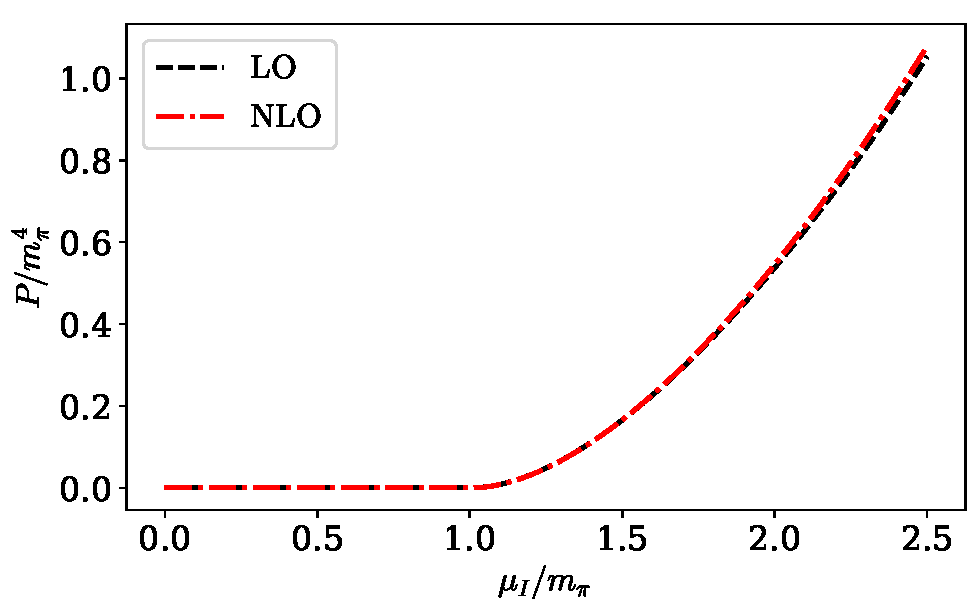
\includegraphics[width=\textwidth]{figurer/numerics/pressure.pdf}
        \caption{The NLO and LO result for the pressure of the pions, as a function of $\mu_I$.}
        \label{fig:pressure}
    \end{subfigure}
    \begin{subfigure}{0.49\textwidth}
        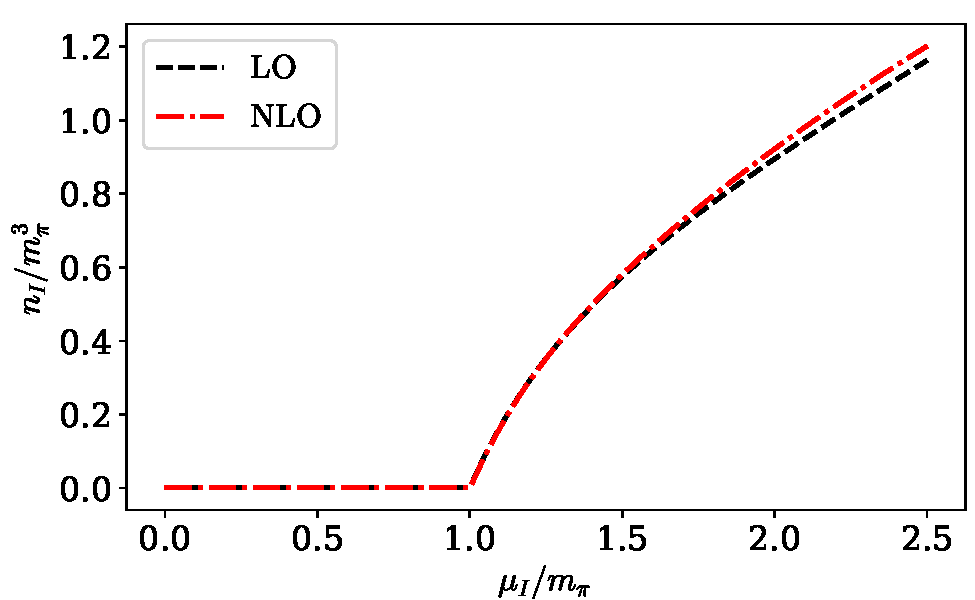
\includegraphics[width=\textwidth]{figurer/numerics/isospin_density.pdf}
        \caption{The NLO and LO result for the isosopin densisty, as a function of $\mu_I$.}
        \label{fig:isospin_density}
    \end{subfigure}
    \caption{}
\end{figure}

These two results can be combined to give the energy density $\mathcal{E}$ as a function of pressure, which is the equation of state.
Energy density is given by 
\begin{equation}
    \mathcal{E} = -P + \mu_I n_I.
\end{equation}
This relationship is shown in \autoref{fig:equation of state}.

\begin{figure}[ht]
    \centering
    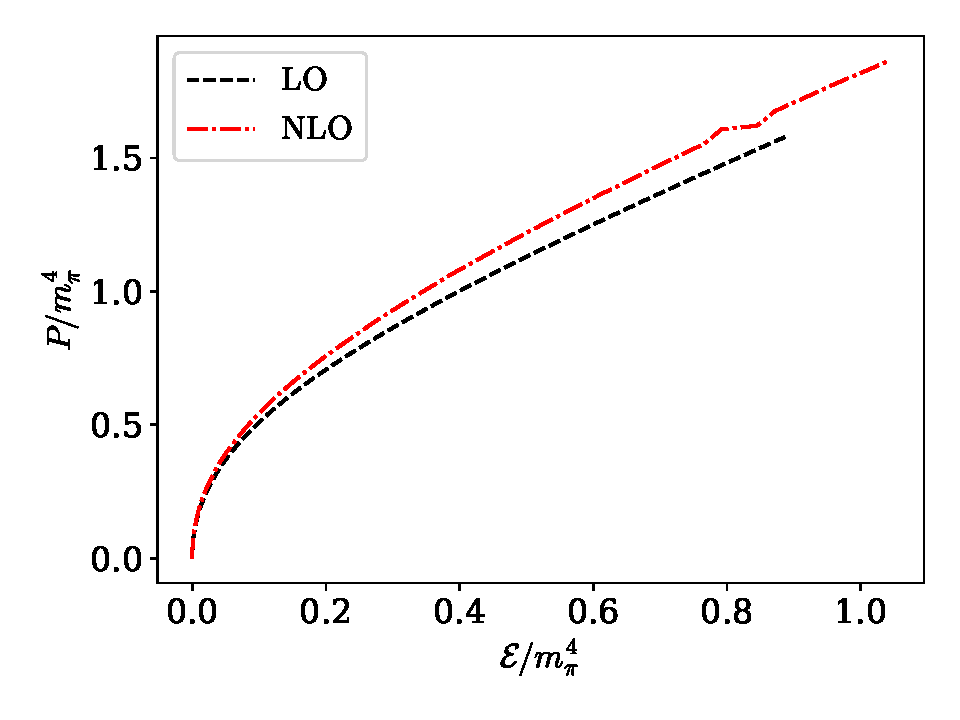
\includegraphics[width=0.7\textwidth]{figurer/numerics/energy_density.pdf}
    \caption{The equation of state of the pions.}
    \label{fig:equation of state}
\end{figure}
